\section{Résultats}

Dans cette dernière section nous allons effectivement aborder le bilan de notre projet en présentant le résultat final obtenu et les diverses améliorations qui pourraient encore être faite sur ce sujet.

\subsection{La solution apportée}

Nous allons donc reprendre tour à tour les différents points présentés dans les parties précédentes et détailler point à point les fonctionnalités réalisées ainsi que la structure finale.

Nous avons donc réussi à atteindre nos objectifs minimaux durant ce projet et même à réaliser certains de nos objectifs supplémentaires. Nous avons réalisé un service web et une application Android qui sont tous les deux versionnés sur GitHub et intégrés en continu grâce à Travis CI qui nous permet de de valider l’intégrité de notre code et de déployer de façon automatique nos solutions. Les différentes versions majeures validées par l’intégration continue sont disponibles sur le site GitHub Releases et le service web est déployé sur une machine privée accessible depuis internet. Notre service web étant de type REST il pourrait être utilisé par différents clients en plus de l’application Android, mais nous n’avons développer que celui-ci par manque de temps c’est pourquoi il n’y a pas d’interface web comme on peut le voir à la figure \ref{archifinale}. Notre service est toutefois pleinement accessible depuis n’importe quel navigateur ou programme pouvant effectuer des requêtes http.

\begin{figure}[H]
    \centering
    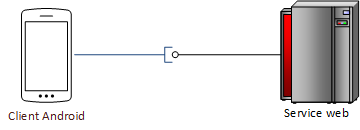
\includegraphics[width=\textwidth]{./img/archi_finale.png}
    \caption{Architecture finale simplifiée}
    \label{archifinale}
\end{figure}

L’architecture est donc assez simple et représente très bien le caractère binaire de notre projet : à savoir une partie serveur universel d’un côté et une partie client lourd de l’autre.

La dernière version de notre solution offre donc les fonctionnalités suivantes. Comme nous pouvons le voir sur la figure \ref{screen1}, nous avons mis en place un logo qui sert d’icône et d’image à notre produit, nous avons aussi une première activité ou vue, permettant la connexion des utilisateurs par le biais de leur compte Google. Comme expliqué dans la section précédente cette activité contacte dans un premier temps les services de Google pour authentifier l’utilisateur courant, pour se faire il faut envoyer l’adresse email, le mot de passe et la clé d’application de WatchDogZZ à Google qui va ensuite renvoyer un jeton en cas de succès. Ce jeton sera alors envoyé pour toutes les communications avec notre service.

\begin{figure}[H]
    \centering
    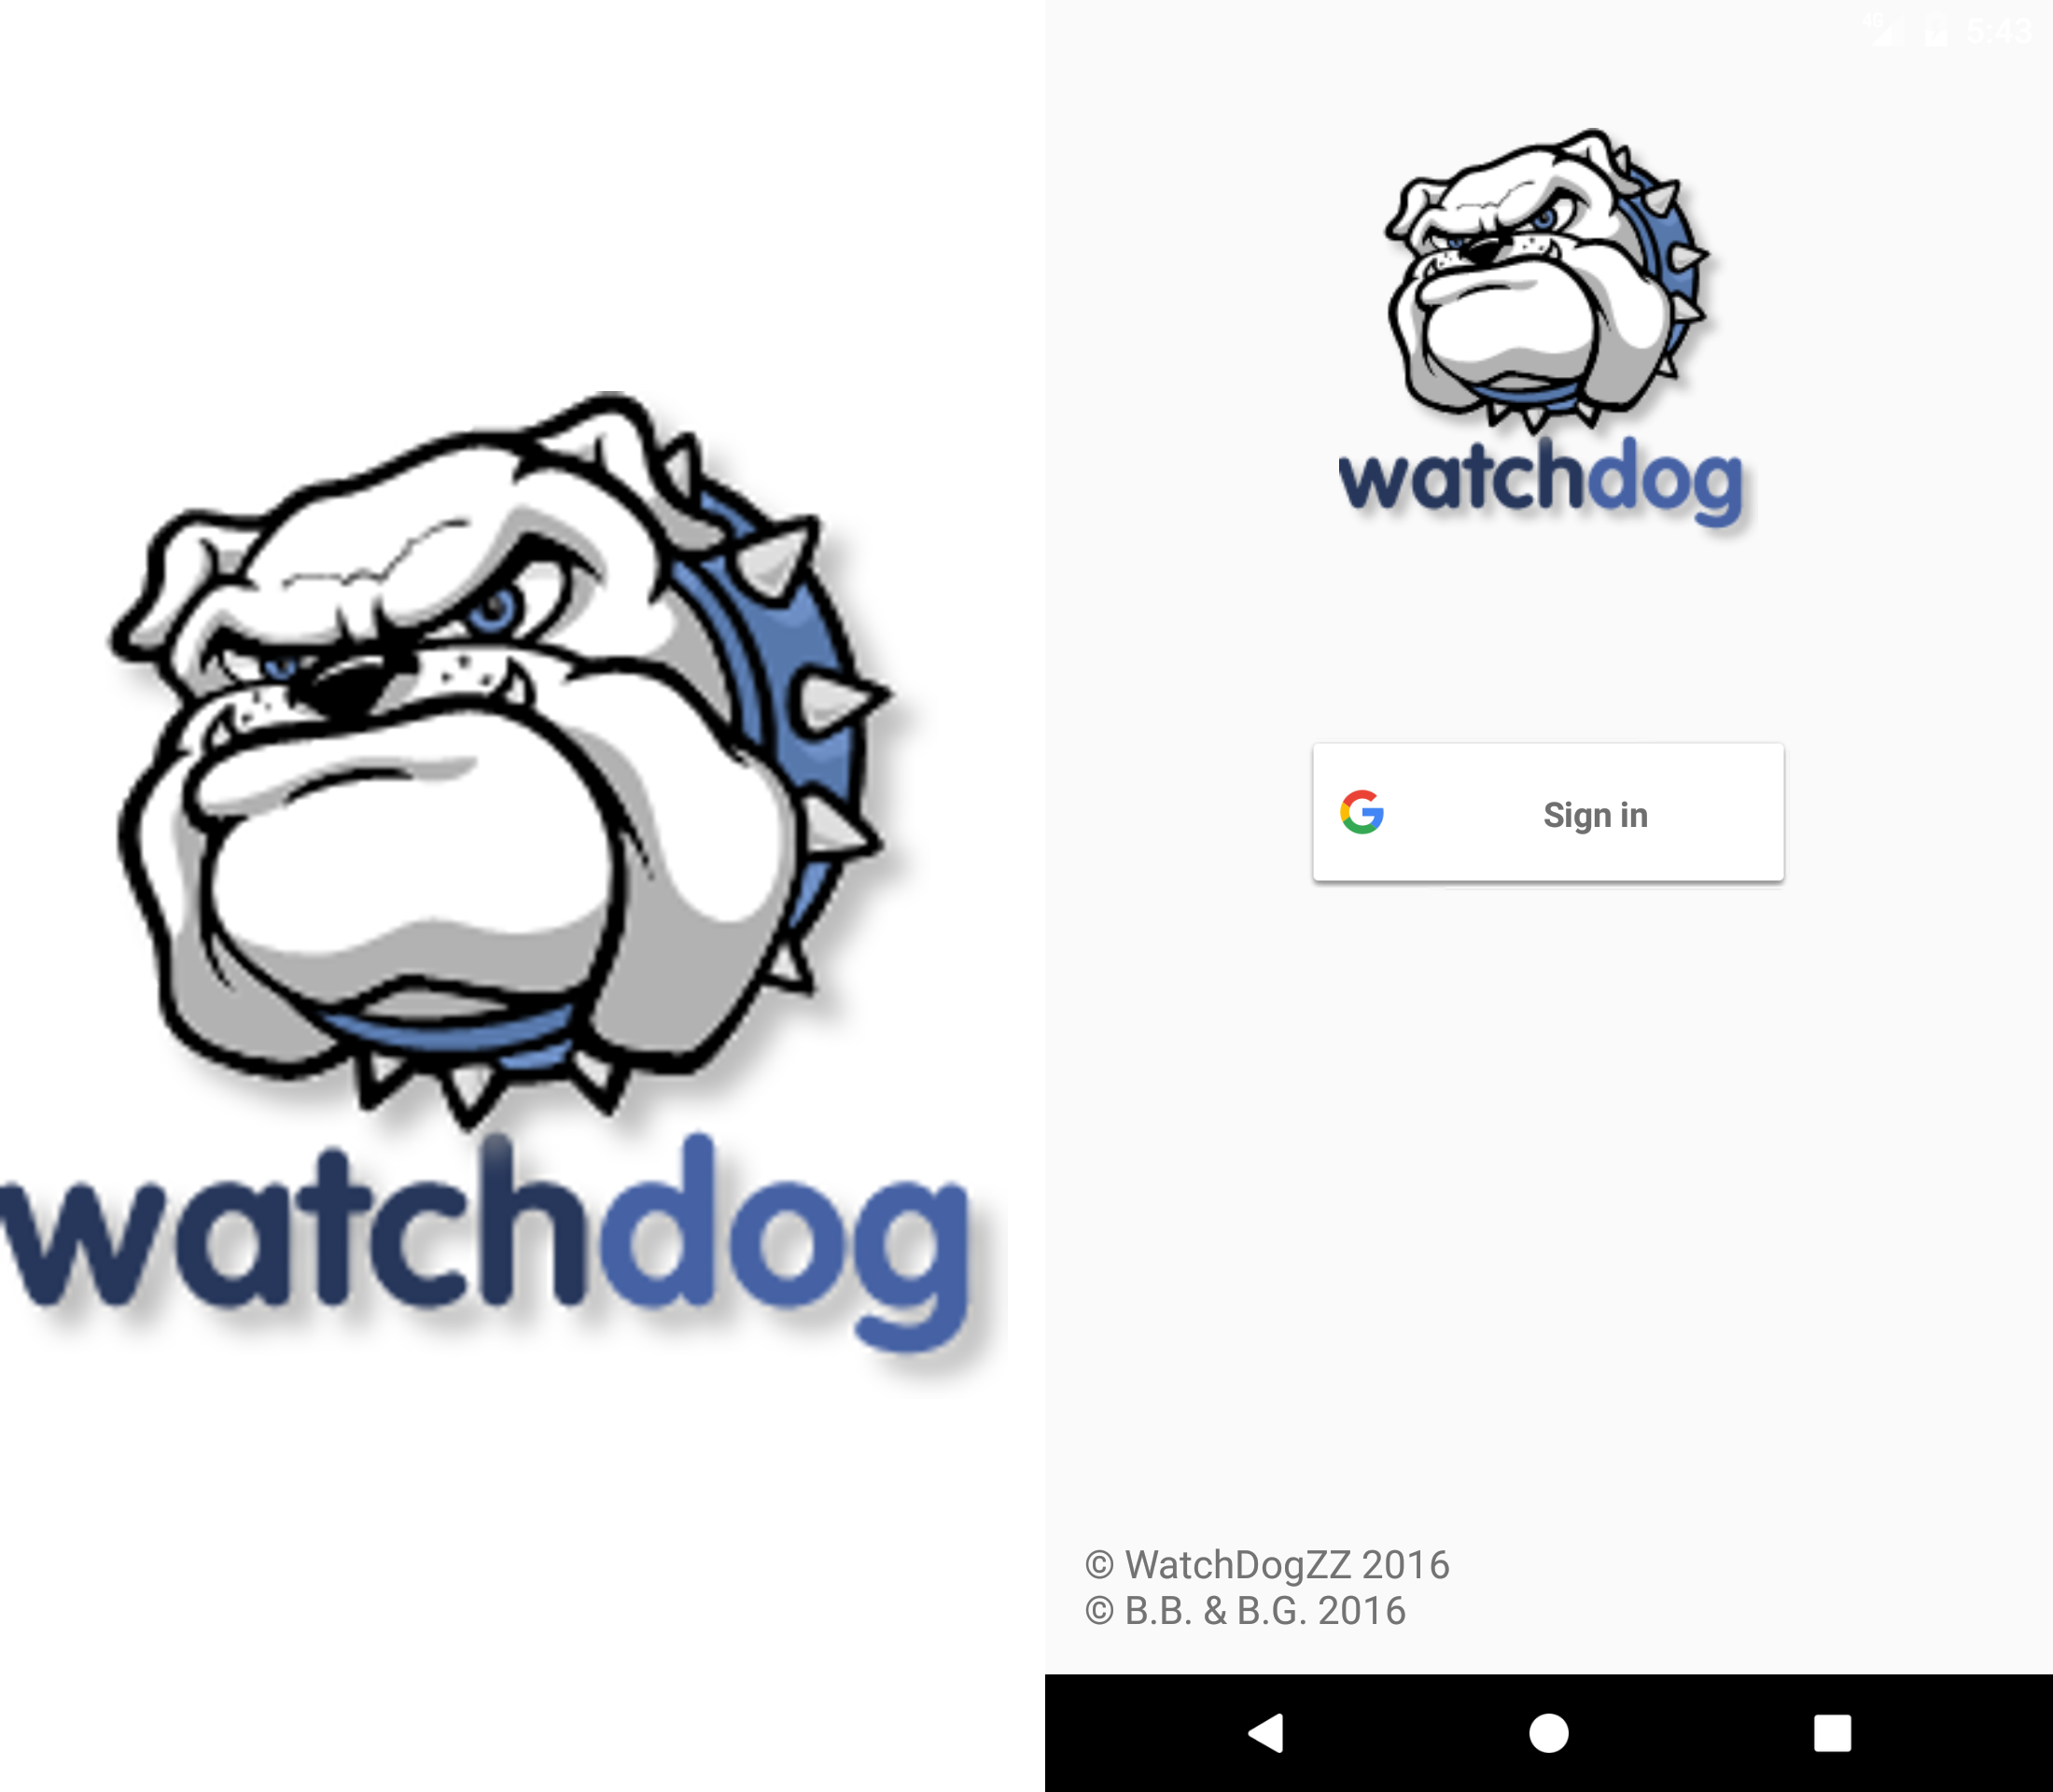
\includegraphics[height=8cm]{./img/screen1.png}
    \caption{Logo et page de connexion de WatchDogZZ}
    \label{screen1}
\end{figure}

Cette première activité est un classique des applications connectées Android moderne et apporte un niveau de fiabilité supérieur à un système d’authentification artisanal.

Une fois cette phase d’authentification passée, l’utilisateur arrive donc sur l’activité principale de l’application : la carte de l’ISIMA. Cette carte en trois dimensions est une simple vue OpenGL où l’arbre de scène du Renderer a été réimplémenté afin d’obtenir les fonctionnalités de navigation et d’affichage voulues de la carte.

Comme on peut le voir sur la figure \ref{screen2}, les différents utilisateurs sont visibles sur la carte, symbolisés par de petites sphères colorées. Leur position se met à jour automatiquement toutes les secondes. Un bouton dans le coin inférieur droit de l’écran permet aussi de positionner des points d’intérêt sur la carte.

L’application dispose d’un menu glissant utilisable en tirant le menu depuis le bord gauche de l’écran. Ce menu donne accès aux différentes fonctionnalités ajoutées comme :

\begin{itemize}
    \item la carte normale ;
    \item la liste des utilisateurs ;
    \item la liste des points d’intérêt ;
    \item le partage de position.
\end{itemize}

Les autres items n’ont pas encore été implémentés, ils n’ont pas été jugés prioritaires en regard des autres fonctionnalités.

\begin{figure}[H]
    \centering
    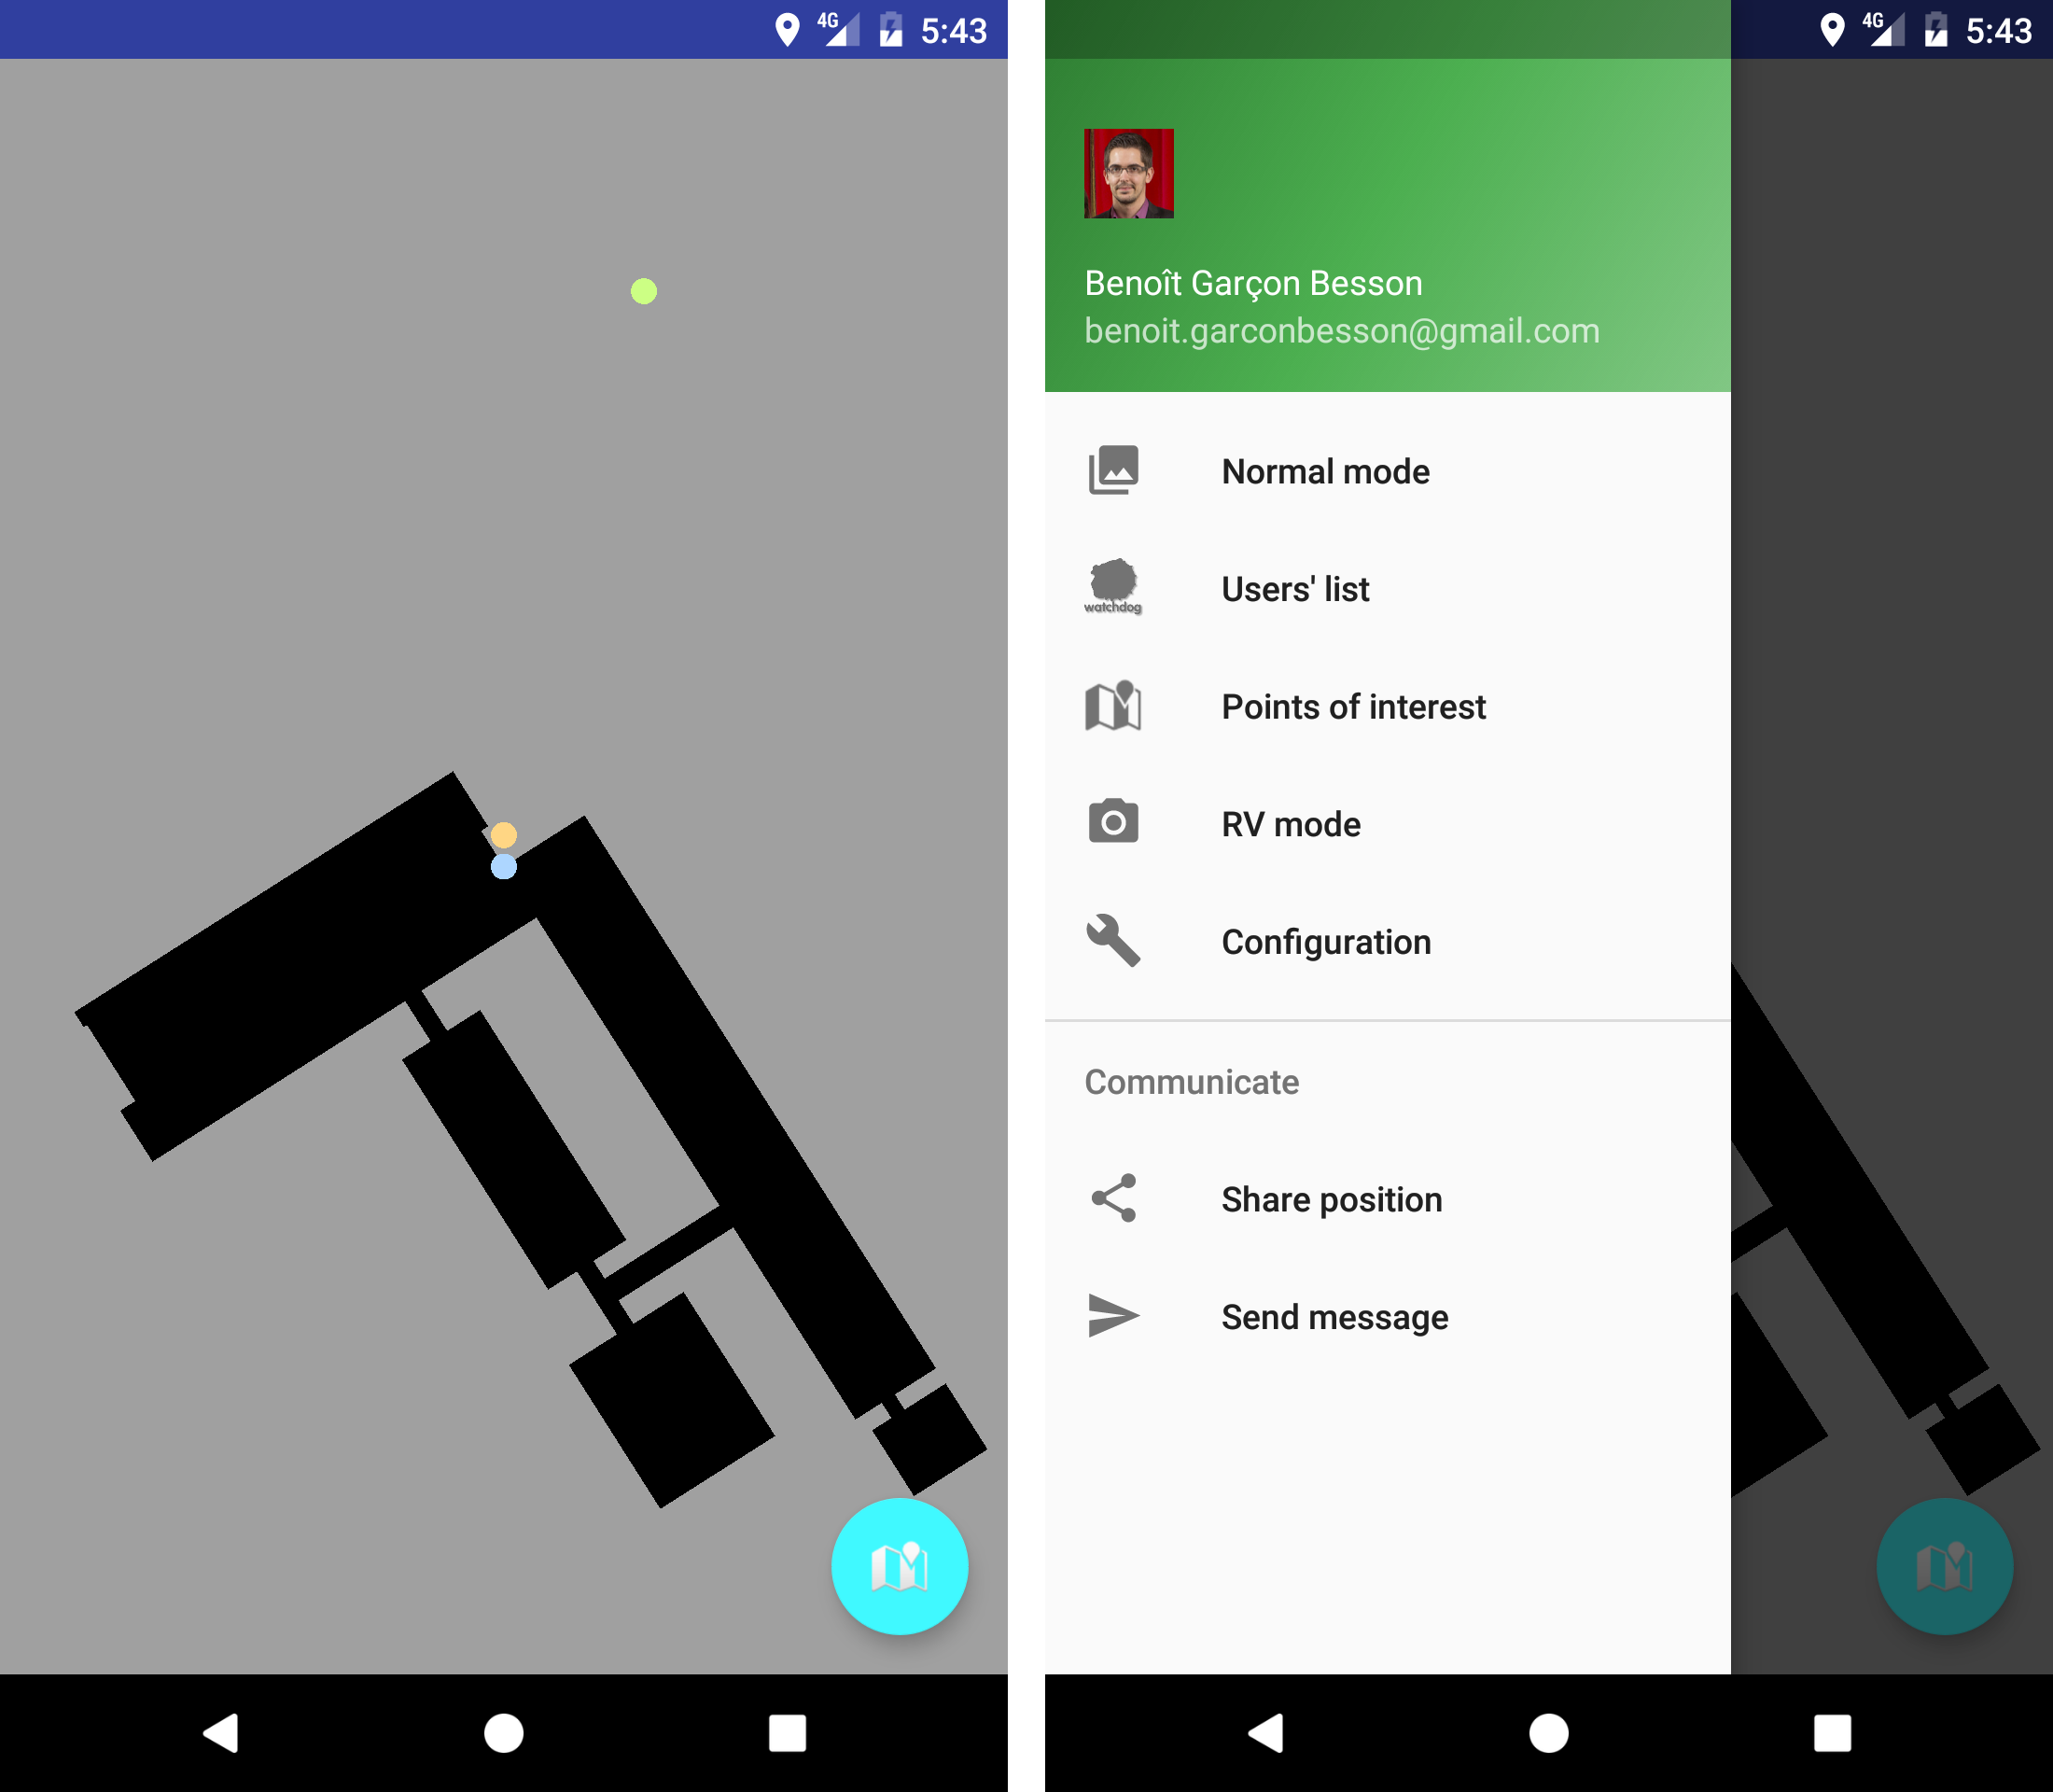
\includegraphics[width=\textwidth]{./img/screen2.png}
    \caption{Vue principale de la carte et menu glissant}
    \label{screen2}
\end{figure}

La liste des utilisateurs permet donc d’identifier plus aisément chaque utilisateur. On dispose comme sur la figure \ref{screen3} de la liste des utilisateurs avec leur photo et leur nom. 

\begin{figure}[H]
    \centering
    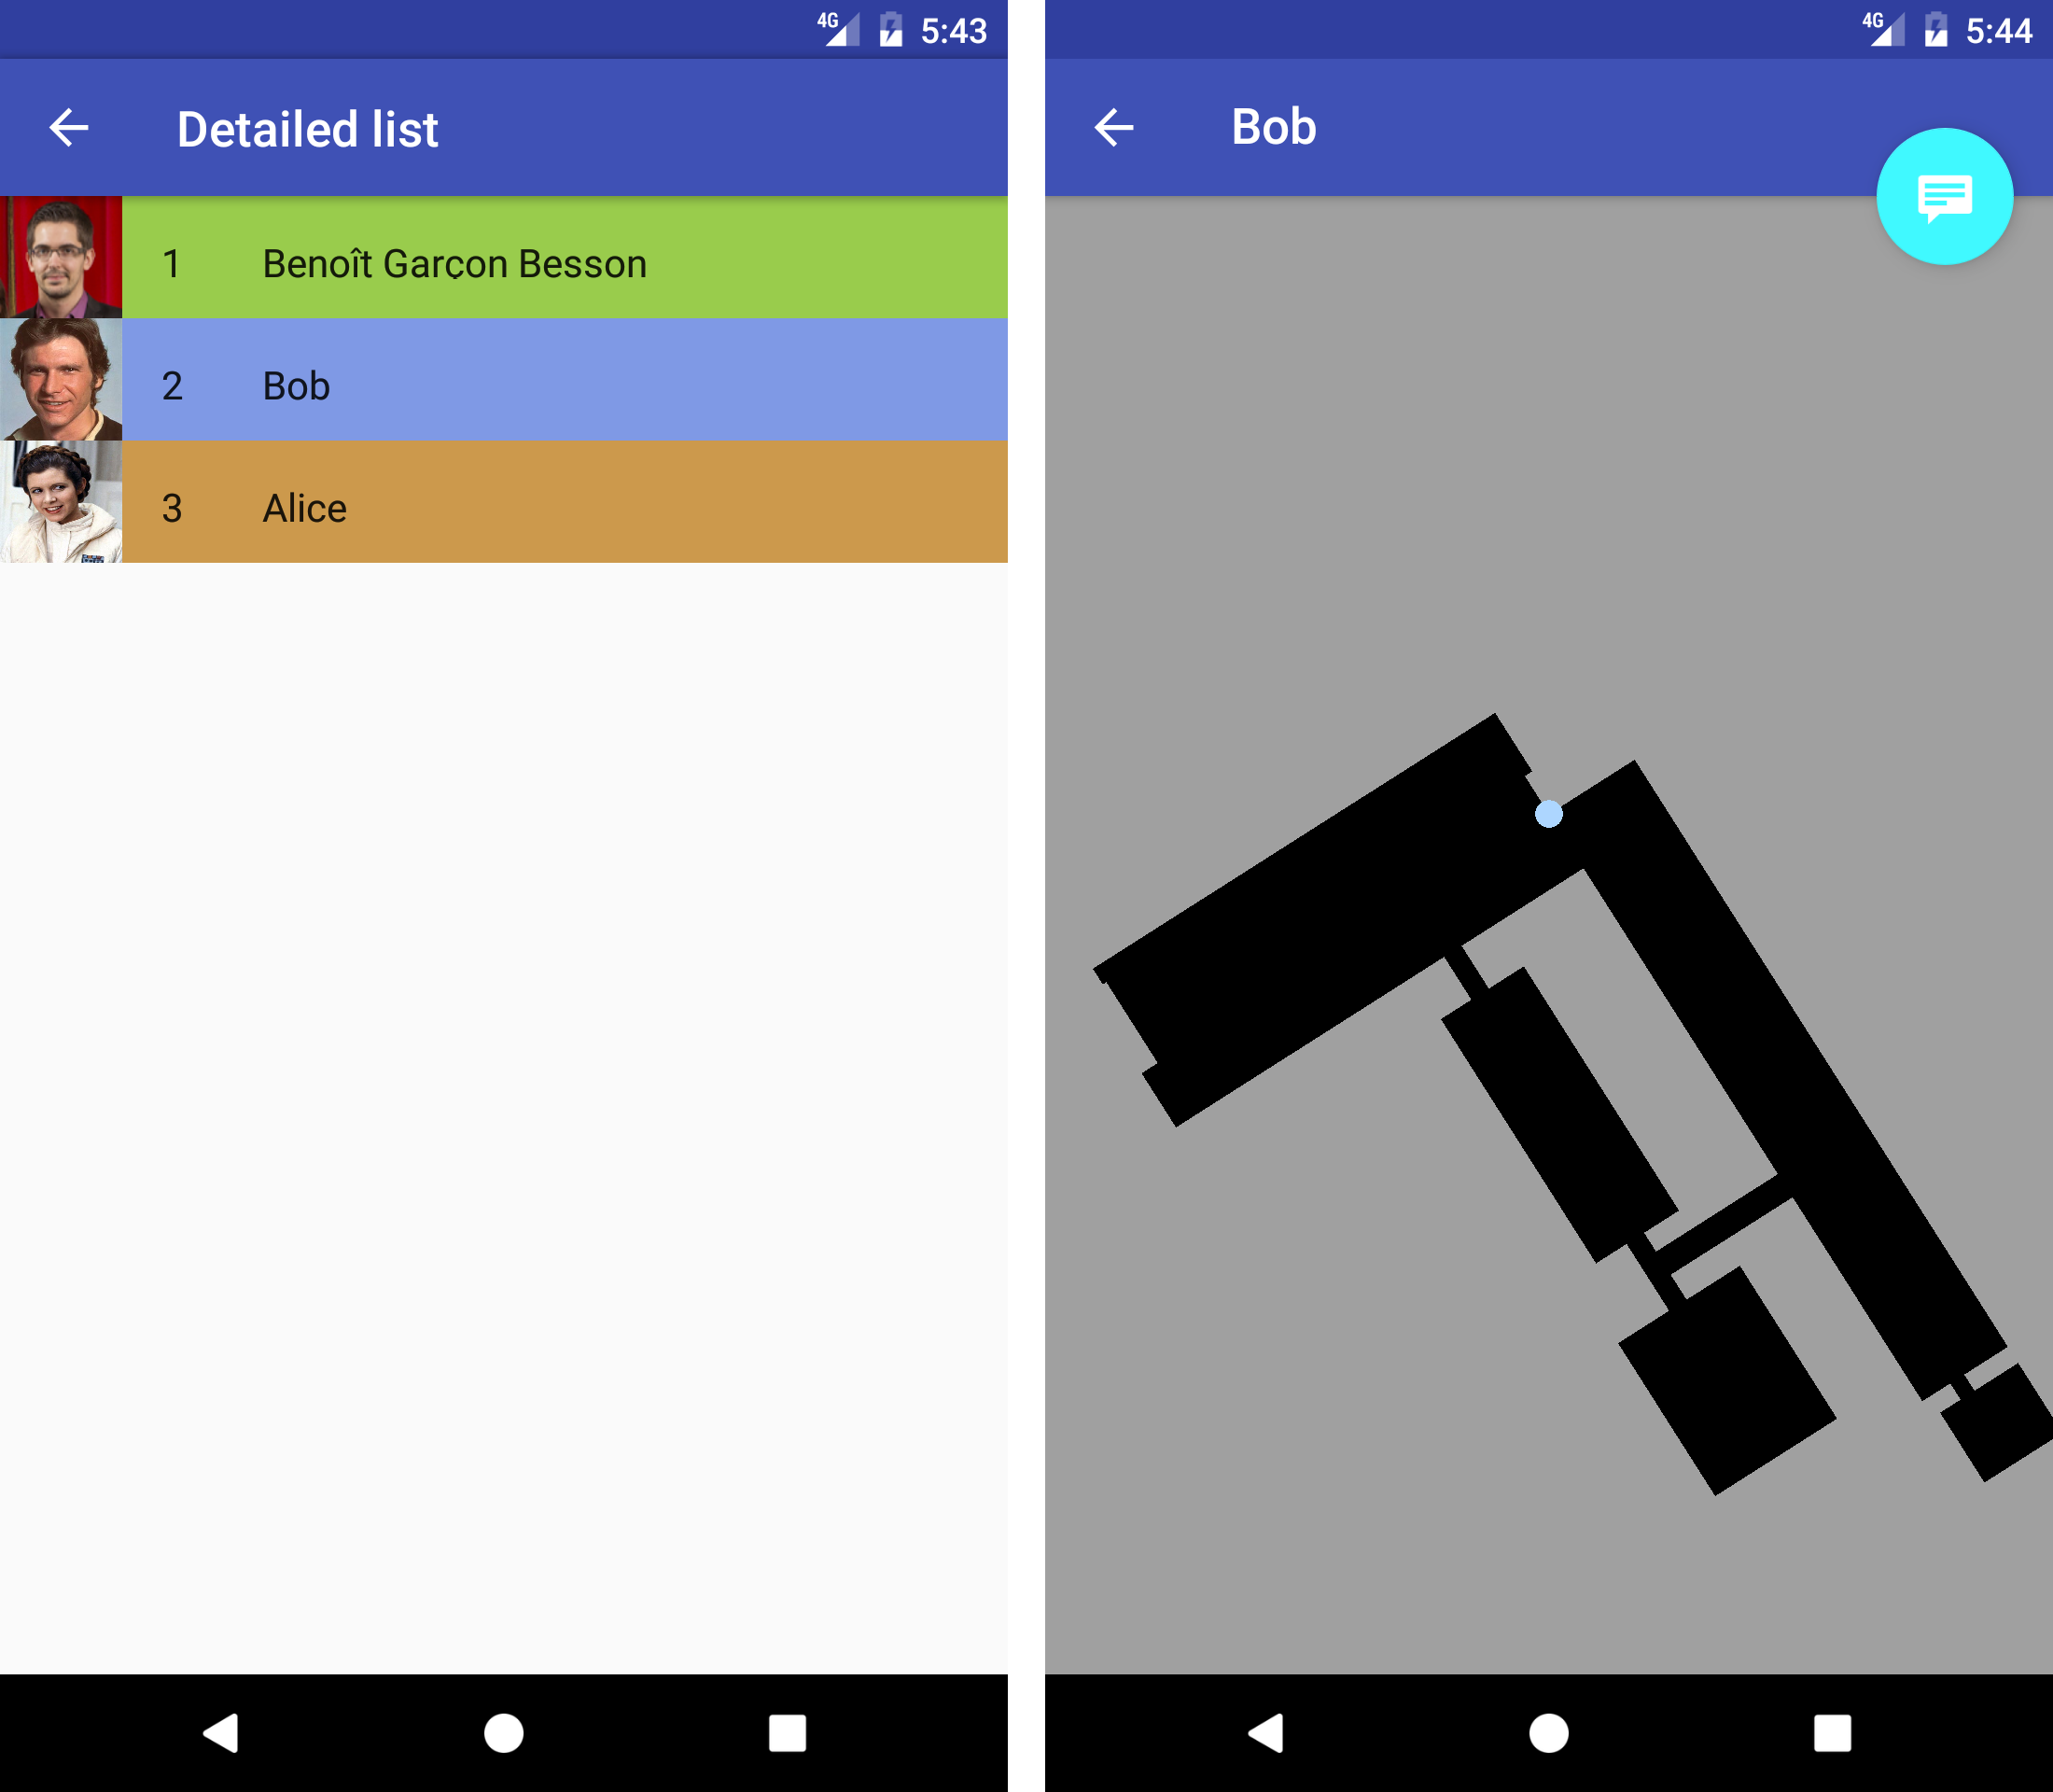
\includegraphics[height=8cm]{./img/screen3.png}
    \caption{Liste détaillée des utilisateurs}
    \label{screen3}
\end{figure}

La couleur associée à chaque utilisateur est issue du hashage de leur nom : ainsi leur couleur dans la liste est la même que celui de leur item sur la carte ce qui nous permet de les identifier. L’algorithme de hashage du nom est très simple et peut se traduire comme sur le code suivant.

\lstset{language=Java}
\begin{lstlisting}[caption=Hashage du nom en couleur]
int hash = label.hashCode();
r = abs((hash % 10)*255/10f/255f);	// calcul de la composante rouge
hash/=10;
g = abs((hash % 10)*255/10f/255f); 	// calcul de la composante verte
hash/=10;
b = abs((hash % 10)*255/10f/255f); 	// calcul de la composante bleue
\end{lstlisting}

De plus en sélectionnant un utilisateur dans la liste, on peut obtenir une carte simplifiée avec seulement le suivi de cette personne pour un suivi plus clair.

Pour en revenir aux points d’intérêt, leur ajout se fait comme dit précédemment par l’utilisation du bouton flottant au bas de l’écran. Cette action invite l’utilisateur à positionner le point vert à l’emplacement désiré et à valider ce placement avec bouton d’ajout. Cette nouvelle action lance un nouveau fragment permettant de nommer se point (figure \ref{screen4}).

\begin{figure}[H]
    \centering
    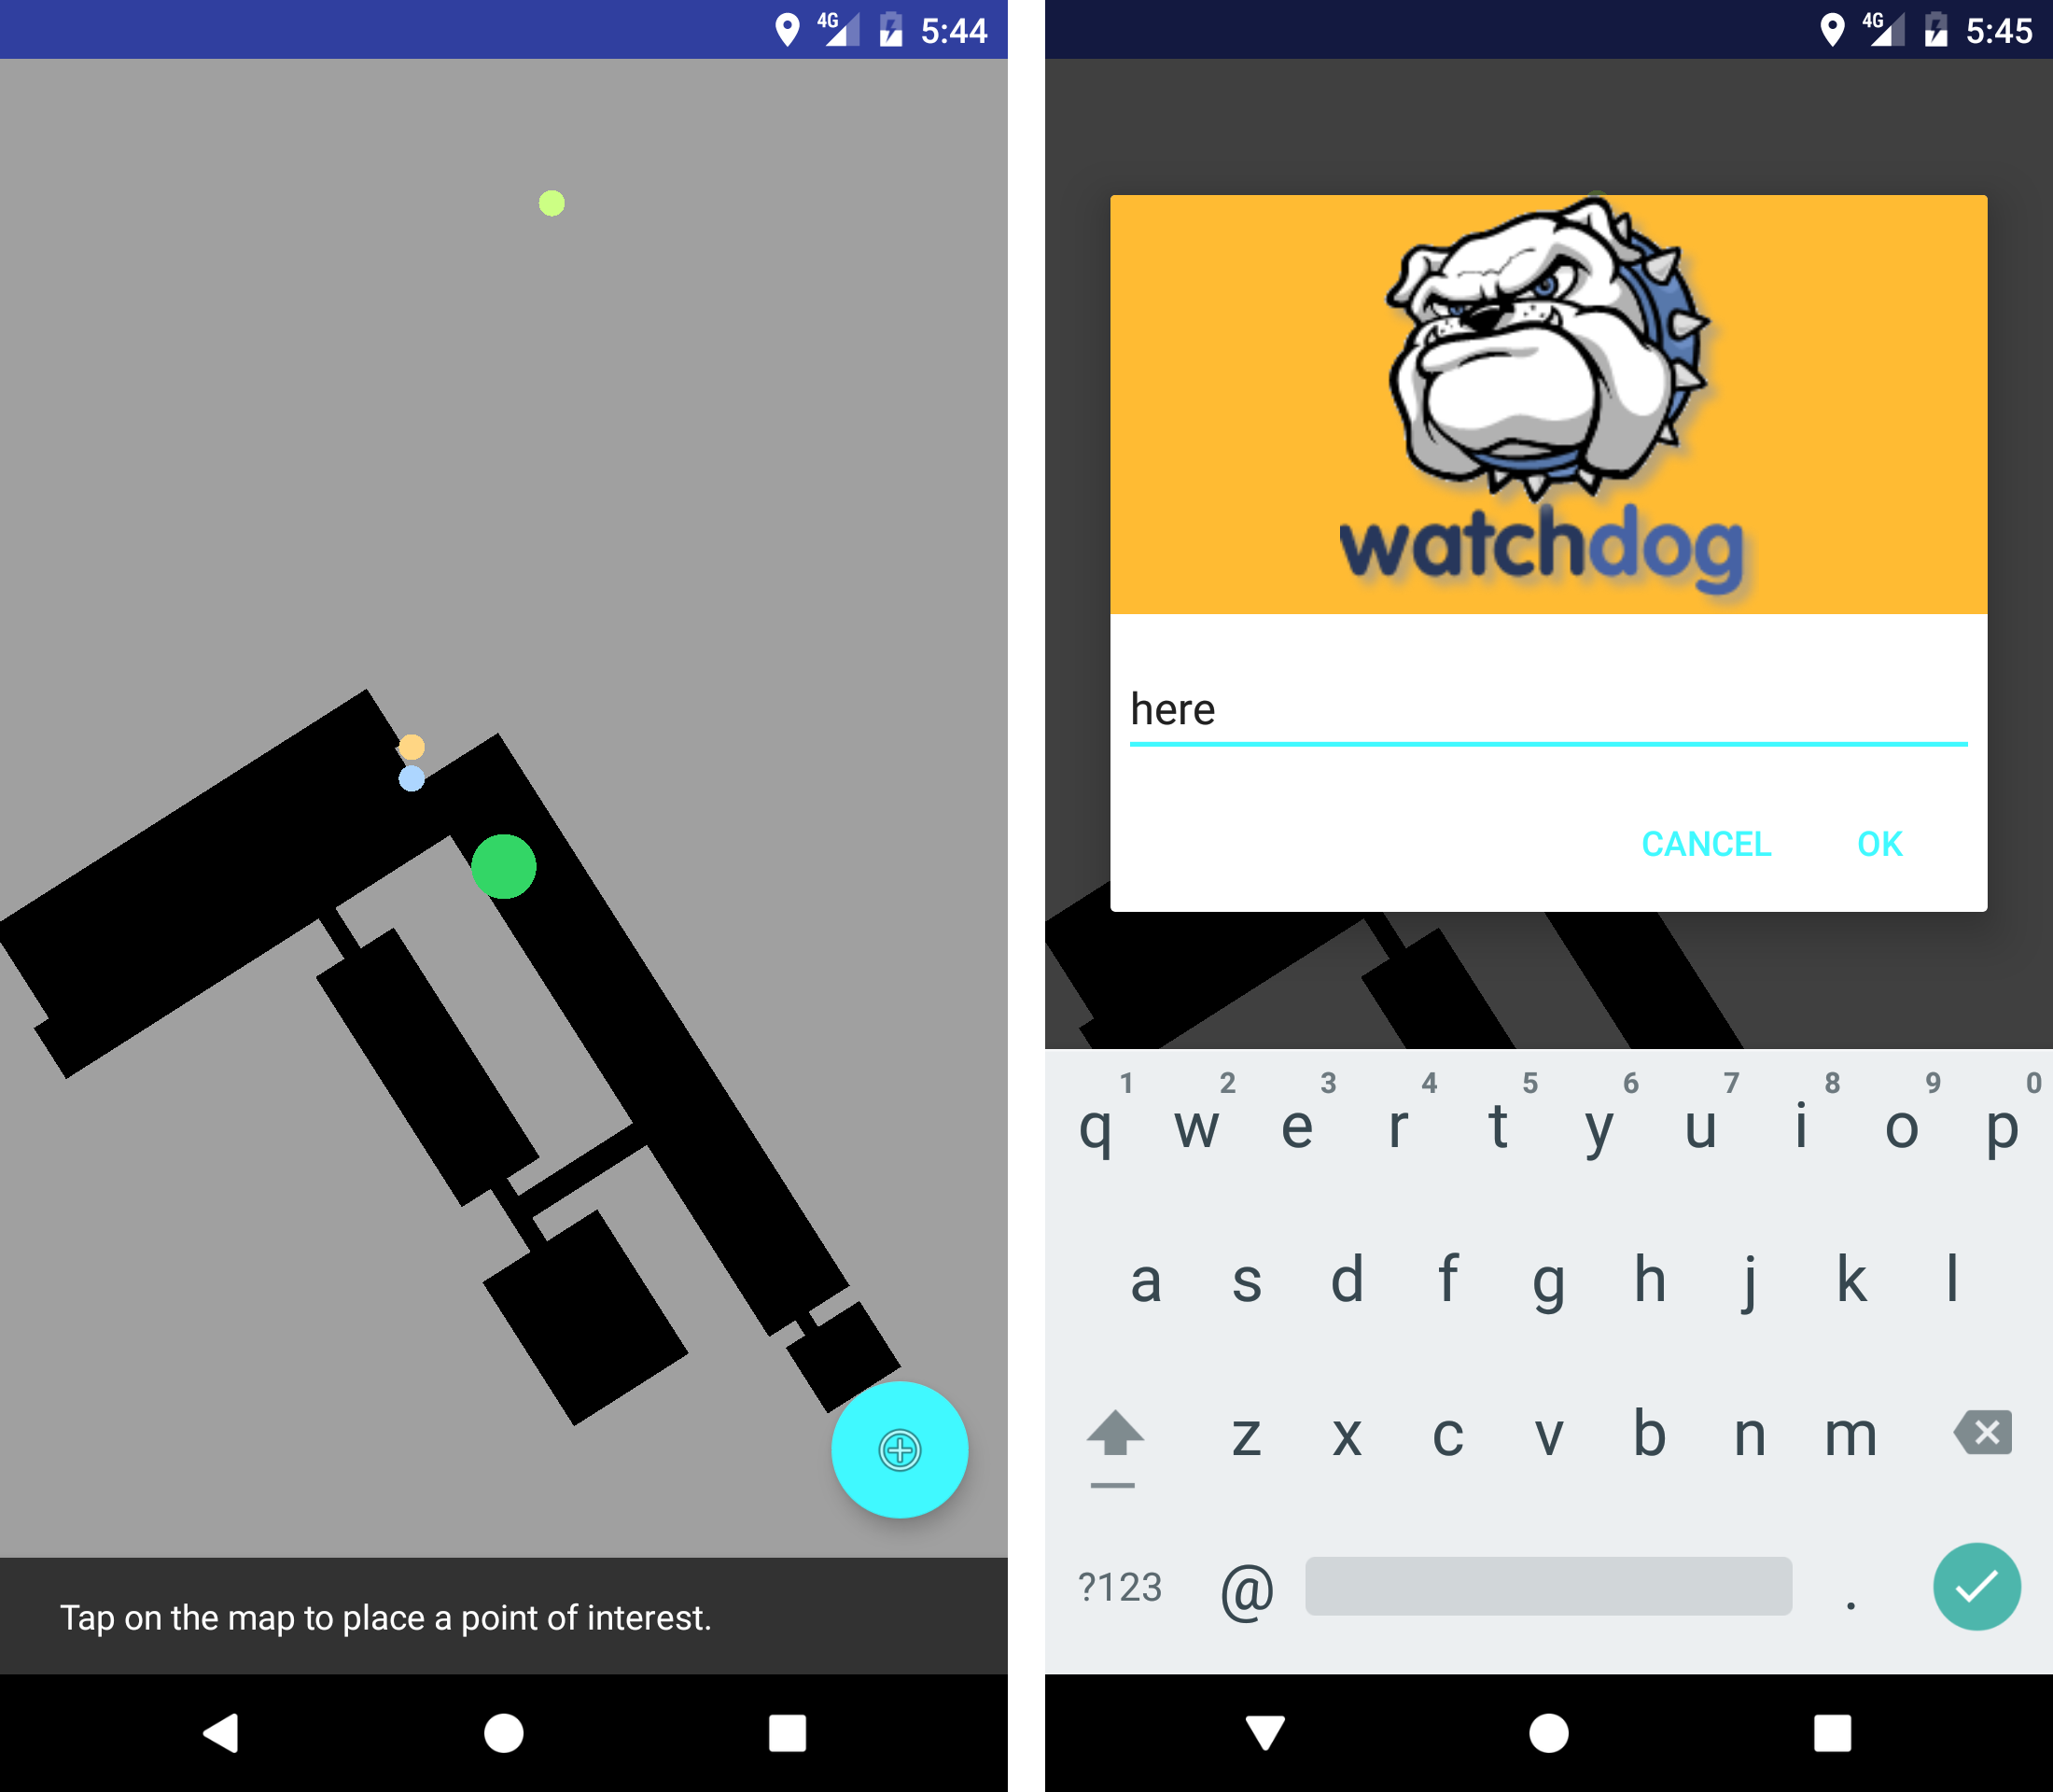
\includegraphics[height=8cm]{./img/screen4.png}
    \caption{Ajout d’un point d’intérêt}
    \label{screen4}
\end{figure}

Ce point est ensuite disponible dans la liste des points d’intérêt qui se base sur les mêmes principes que la liste d’utilisateurs. Comme on peut le voir sur la figure \ref{screen5}, une couleur est associée associer à chaque point par rapport à son nom et il est possible d’afficher le point sur la carte en le sélectionnant dans la liste.

\begin{figure}[H]
    \centering
    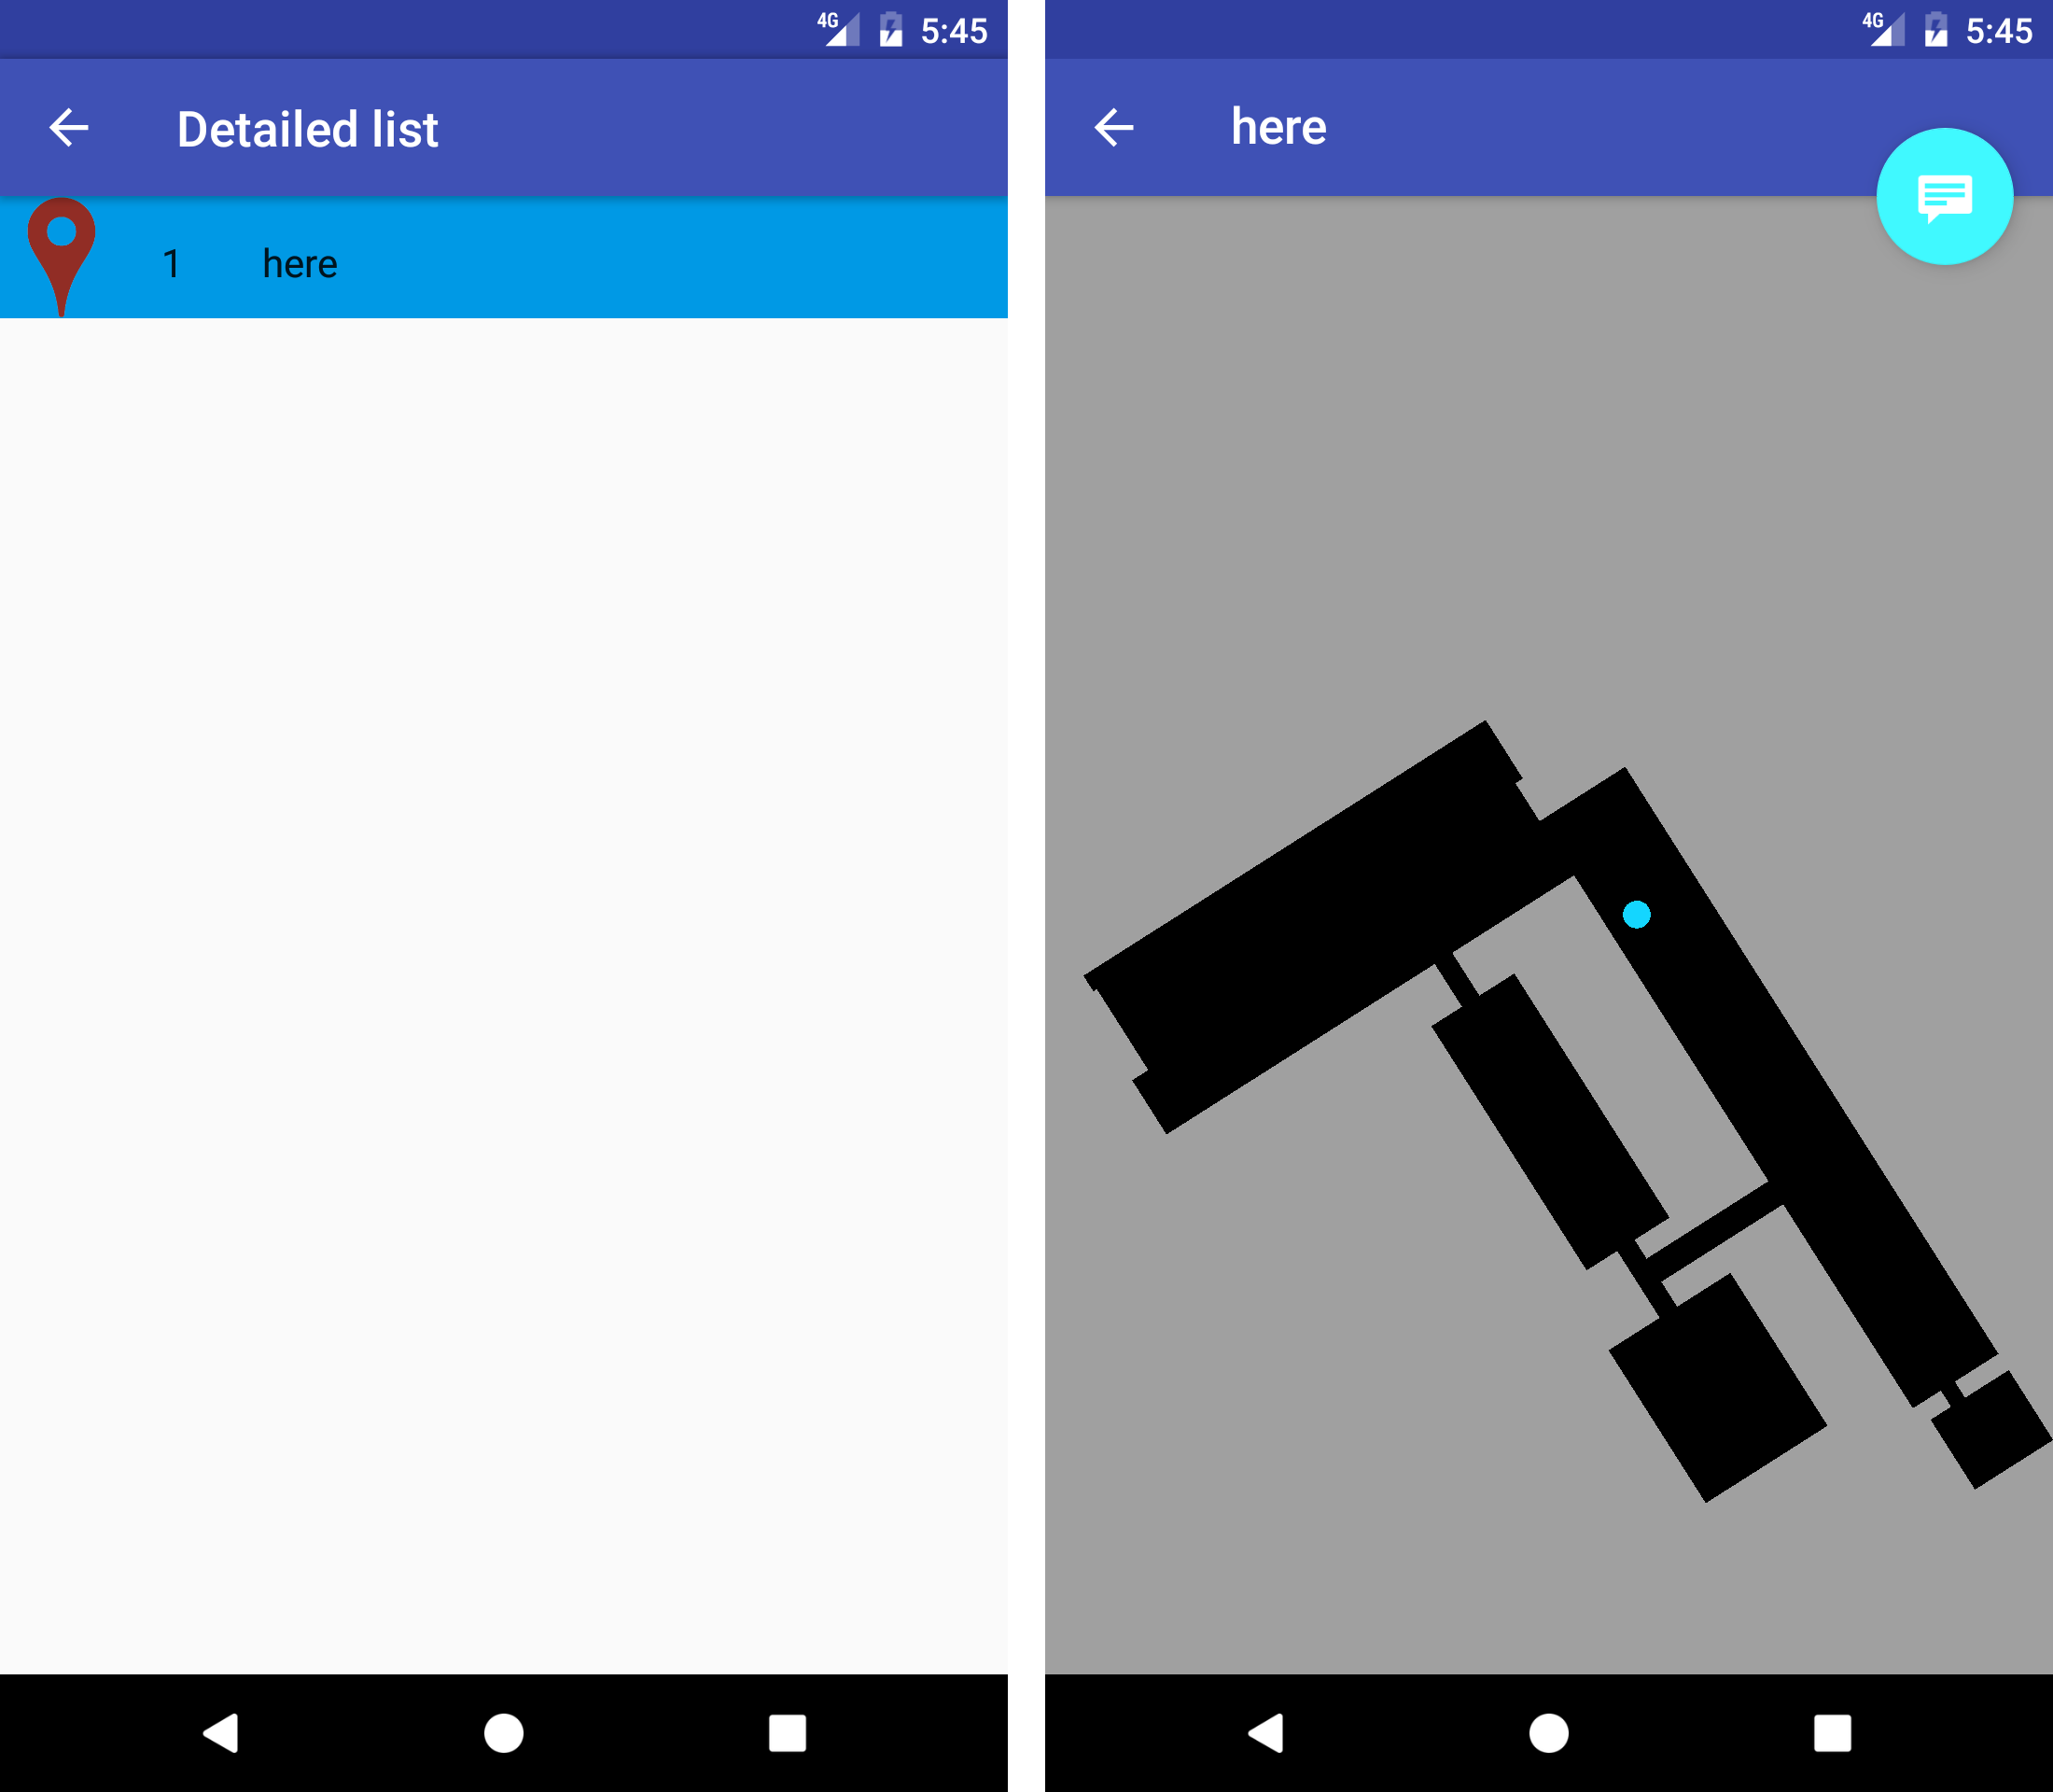
\includegraphics[height=8cm]{./img/screen5.png}
    \caption{Liste détaillée des points d’intérêt}
    \label{screen5}
\end{figure}

Toutes ces fonctionnalités nécessitent l’utilisation du serveur, mais la dernière, le partage de position est une fonctionnalité qui permet de s’affranchir du service web puisqu’il permet d’envoyer sa position à n’importe qui par n’importe quel moyen de communication. Ceci est rendu possible par les intents Android. Les intents sont des descriptions d’une action à effectuer et pouvant comporter des données nommées. Les intents sont produits par les applications pour être dirigées par le système Android vers l’application la plus capable d’effectuer l’action et en cas de choix multiple, la décision est donnée à l’utilisateur. Ainsi en produisant un intent devant envoyer le texte comportant notre position n’importe quel processus de type messagerie SMS, email ou autre peut l’envoyer : c’est au choix de l’utilisateur. On peut donc utiliser l’application même en cas de problème de communication avec le serveur.

Enfin concernant les communications avec le serveur, celles-ci sont sécurisées puisqu’elles utilisent le protocole https. Il a fallu pour ce faire créer un certificat pour le serveur enregistré auprès d’un service de certification et ensuite ajouter ce service de certification auprès des services de confiance de l’application. Au final ceci permet d’échanger avec le serveur toutes les informations personnelles nécessaires en garantissant la sécurité minimale.

Concernant les performances du service, elles semblent plutôt bonnes pour un nombre limité d’utilisateur. La position du terminal courant peut être récupérée à une fréquence au moins égale à la fréquence d’affichage sur le service gps et celles des autres ne nécessitent que quelques dizaines de millisecondes ce qui est plutôt convenable pour des appels réseaux répétés. Toutefois nous n’avons pas d’information sur le comportement de notre service à une échelle plus réaliste c’est-à-dire avec un nombre d’utilisateur représentatif d’une situation réelle.

Nous avons vu toutes les fonctionnalités disponibles sur notre solution mais il en existe de nombreuses autres que nous n’avons pas pu développer et certains points pourraient aussi être améliorés.

\subsection{Améliorations possibles}

Bien que l'application WatchDogZZ soit à l'heure actuelle une application complète et répondant à nos attentes, ce projet reste un sujet très vaste et très ouvert sur lequel il est possible de faire énormément.